\section{Introduction à l'électronique}
\subsection{Définition de quelques termes}
\begin{flushleft}
    Avant toute chose, nous allons définir assez simplement quelques termes concernant le matériel que nous allons utiliser:\\\vskip0.4cm
    Servomoteur : Sa fonction principale est d'assurer la reproduction d'un mouvement en réponse à une commande externe. En l'occurence la commande sera envoyée par nos potentiomètres linéaires.\\
    
    \begin{multicols}{2}
    
\includegraphics[width=60pt,height=60pt]{Déroulé/Jour_1/Manuel d'utilisation/Images/6.jpg}
    
    \columnbreak
    
    \textbf{\large Attention : }\textbf{\textit{ Les servomoteurs que nous utilisons ici sont des servomoteurs standards et ont une plage de mouvement entre 0° et 180°.}}\\\vspace{0.2cm}
    \end{multicols}

    Potentiomètre linéaire : Un potentiomètre linéaire est une résistance variable permettant d'ajuster la valeur de certains paramètres. En l'occurence le paramètre ajusté sera la position angulaire du servomoteur correspondant.\\\vspace{0.2cm}
    
    Câbles Dupont mâle-mâle : Ces câbles permettent de créer une connexion sur une platine d'essai sans avoir à réaliser de soudure. Ils sont dits "mâles-mâles" car ils présentent de chaque côté une petite pointe venant s'insérer dans les ports de connexions.\\\vspace{0.2cm}
    
    Platine d'essai (Breadboard en anglais) : Dispositif permettant de réaliser le prototypage et le test d'un circuit électronique sans avoir à réaliser de soudure.\\\vspace{0.2cm}
    
    Entrée digitale : \'Egalement appelée entrée numérique. Ce sont des entrées ne pouvant prendre que 2 valeurs : 0 (le système est à l'arrêt) et 1 (le système est en fonctionnement).\\\vspace{0.2cm}
    
    Entrée analogique : Elle s'oppose à l'entrée digitale et permet de recueillir un signal électrique variable sur une plage de valeur définie au préalable.
\end{flushleft}

\subsection{Ce que l'on utilise pour cet atelier }
\begin{flushleft}
    Pour programmer le mouvement de cette main, nous allons utiliser le matériel suivant :\\
    \begin{figure}[!h]
        \centering
        \begin{tabular}{|l|l|}
            \hline Type & Quantité/unité\\
            \hline Carte Arduino Uno & 1\\
            \hline Câbles Dupont mâle-mâle & 32\\
            \hline Potentiomètres linéaires 10k$\Omega$ & 5\\
            \hline Servomoteurs 9g SG-90 & 5\\
            \hline Platine d'essai & 1\\
            \hline Pile 9V & 1\\
            \hline Support de pile (banchement sur port secteur) & 1\\
            \hline
        \end{tabular}
        \caption[Matériel électronique]{Liste du matériel électronique nécessaire}
        \label{2.1}
    \end{figure}
\end{flushleft}

%provisoire
\newpage

\subsection{Fonctionnement des composants}

\begin{flushleft}
    \textbf{La platine d'essai :}\vspace{0.4cm}
    \begin{figure}[!h]
        \centering
        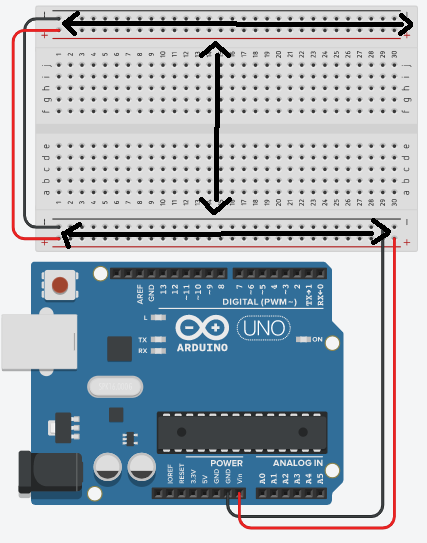
\includegraphics[height=300pt]{Déroulé/Jour_2/breadboard.PNG}
        \caption[Platine d'essai]{Sens des connexions sur la platine d'essai}
        \label{2.2}
    \end{figure}

    \textbf{La carte Arduino :}\vspace{0.4cm}
    \begin{figure}[!h]
        \centering
        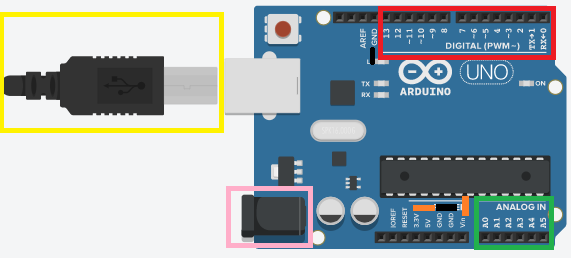
\includegraphics[width=300pt]{Déroulé/Jour_2/Carte.PNG}
        \caption[Carte Arduino]{Description des différents ports de la carte Arduino}
        \label{fig:my_label}
    \end{figure}
    \end{flushleft}
    
    %provisoire
    \newpage
    
    \begin{flushleft}
    \underline{\textit{\large Légende :}}\vspace{0.4cm}

    \begin{itemize}
        \item \begin{flushleft}\textcolor{orange}{Traits orange :} Ce sont les ports de la carte permettant d'alimenter en tension la platine d'essai. Cette carte présente une alimentation en 3.3V, une en 5V et celle qui va nous intéresser étant donné que nous allons alimenter l'Arduino avec une pile 9V : $V_{in}$.\vspace{0.2cm}
        \end{flushleft}
        \begin{flushleft}
        \begin{multicols}{2}
        
\includegraphics[width=60pt,height=60pt]{Déroulé/Jour_1/Manuel d'utilisation/Images/6.jpg}
    
        \columnbreak
    
        \textbf{\large Attention : }\textbf{\textit{ La carte Arduino Uno peut supporter une tension d'alimentation externe entre 6V et 20V mais il est recommandé que cette tension soit comprise entre 7V et 12V.}}\\\vspace{0.2cm}
        \end{multicols}
        \end{flushleft}
        
        \item \textcolor{black}{Traits noir :} Ce sont les ports de la carte permettant de mettre les différents composants branchés à la masse (= gnd sur la carte $\Leftrightarrow$ ground en anglais). Cela correspond à une tension de 0V.\vspace{0.2cm}
        
        
\includegraphics[width=30pt,height=30pt]{Déroulé/Jour_1/idée.png}
        \textbf{\large Astuce : }\textbf{\textit{\large En pratique, lorsque l'on utilise une platine d'essai, on connecte un des ports de masse de l'Arduino à la ligne de masse de la platine d'essai avec un câble Dupont (Voir figure 15).}}\\\vspace{0.2cm}
        
        \item \textcolor{yellow}{Carré jaune :} C'est le port d'alimentation en USB de la carte Arduino. Il permet de téléverser le programme de l'ordinateur sur le microprocesseur de la carte, et également de l'alimenter si on le laisser branché une fois le programme téléversé.\\\vspace{0.2cm}
        
        \item \textcolor{pink}{Carré rose :} C'est le port d'alimentation sur secteur de l'Arduino. C'est celui qui va nous permettre d'alimenter la carte lors de notre projet.\\\vspace{0.2cm}
        
        \item \textcolor{green}{Carré vert :} Ce sont les ports d'entrées analogiques de la carte. Ici ils vont nous servir à brancher les différents potentiomètres.\\\vspace{0.2cm}
        
        \item \textcolor{red}{Carré rouge :} Ce sont les ports d'entrées digitales de la carte. Ici ils vont nous servir à brancher les différents servomoteurs.\vspace{0.2cm}
    \end{itemize}
    
    %provisoire
    \newpage
    
    \textbf{Les potentiomètres :}\vspace{0.4cm}
    \begin{figure}[!h]
        \centering
        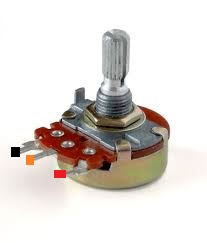
\includegraphics[]{Déroulé/Jour_2/potentiomètre.jpg}
        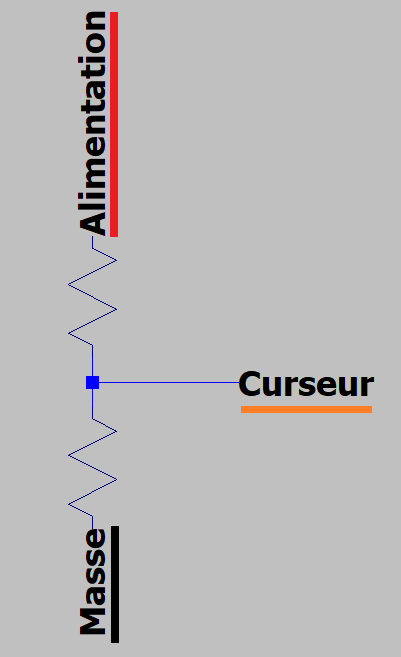
\includegraphics[width=100pt]{Déroulé/Jour_2/schéma_potentiomètre.PNG}
        \caption[Potentiomètre]{Photo et schéma électronique d'un potentiomètre linéaire}
        \label{2.4}
    \end{figure}
    \begin{flushleft}
    \underline{\textit{\large Légende :}}\vspace{0.4cm}
    
        \begin{itemize}
    \item \textcolor{black}{Point et trait noir :} Port relié à la masse de la platine d'essai.\vspace{0.2cm}
    \item \textcolor{red}{Point et trait rouge :} Port relié à l'alimentation de la platine d'essai.\vspace{0.2cm}
    \item \textcolor{orange}{Point et trait orange :} Port relié au curseur du potentiomètre et à l'entrée analogique de l'Arduino, permettant de lire la valeur du potentiomètre.
    \end{itemize}
    \end{flushleft}
    
    Dans notre cas, faire bouger le curseur du potentiomètre va permettre d'envoyer une certaine valeur de tension au servomoteur en la convertissant en une position angulaire (entre 0° et 180°). Cette position sera alors lue par le servomoteur qui bougera jusqu'à atteindre la position demandée.\\
    \end{flushleft}
    
    \begin{flushleft}
    \textbf{Le servomoteur SG-90 :}\vspace{0.4cm}
    \end{flushleft}
    \begin{figure}[!h]
        \centering
        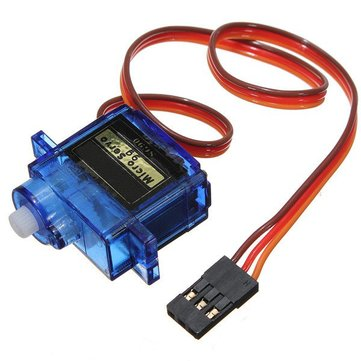
\includegraphics[width=150pt,height=150pt]{Déroulé/Jour_2/SG90.jpg}
        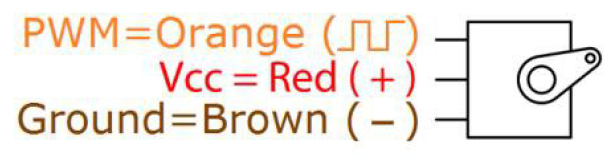
\includegraphics[width=300pt]{Déroulé/Jour_2/schéma_SG90.PNG}
        \caption[Servomoteur SG-90]{Photo et schéma du servomoteur utilisé}
        \label{2.5}
    \end{figure}
    
    \begin{flushleft}
    \textbf{\large Note : }\textbf{\textit{ PWM (= Pulse With Modulation en anglais) correspond à une entrée digitale sur l'Arduino.}}\\\vspace{0.2cm}
    \end{flushleft}
    
    %provisoire
    \newpage
    
    \begin{flushleft}
    \textbf{La pile :}\vspace{0.4cm}
    \end{flushleft}
    \begin{figure}[!h]
        \centering
        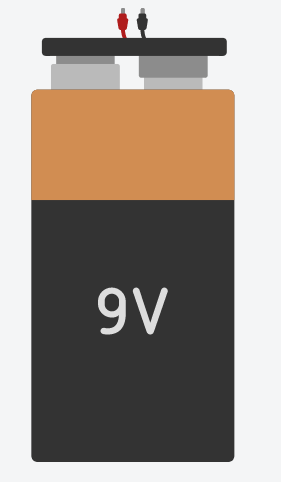
\includegraphics[height=200pt]{Déroulé/Jour_2/pile.PNG}
        \caption[Pile]{Schéma de la pile 9V}
        \label{fig:my_label}
    \end{figure}
    \begin{flushleft}
    \underline{\textit{\large Légende :}}\vspace{0.4cm}
    
    \begin{itemize}
    \item \textcolor{red}{Câble rouge :} Câble d'alimentation 9V de la pile (borne +).\vspace{0.2cm}
    \item \textcolor{black}{Câble noir :} Câble de masse de la pile (borne -).
    \end{itemize}
    \end{flushleft}
    
\subsection{Où acheter son matériel ?}

\begin{flushleft}
     Il est très facile de vous procurer le matériel. Il y a énormément de sites et/ou magasins spécialisés dans la vente de composants électroniques pour les particuliers. Un grand nombre de composants sont également disponibles sur des sites comme Amazon, Ebay, etc..
\end{flushleft}
